\section*{Methodology}

\subsection*{PyKEEN}

PyKEEN~\cite{pykeen} is an open-source Python library that facilitates training and evaluation of knowledge graph embedding models.
It streamlines the process of embedding entities and relations into continuous vector spaces, enabling efficient link prediction and relationship classification.
PyKEEN supports a wide range of models, including TransE, RotatE, ComplEx, and DistMult, each with unique characteristics and performance profiles.

In this project, PyKEEN was used to predict missing links within a knowledge graph through a structured workflow involving data extraction, preparation, model training, and link prediction.

\subsection*{Knowledge Graph Embeddings for Link Prediction}

In our experiments, we focused on two primary approaches for knowledge graph completion: traditional knowledge graph embedding models and LLM-based embeddings.
Among knowledge graph embedding models available in PyKEEN, in this first iteration we used several families of models starting from the simplest approaches.
\begin{itemize}
    \item \textbf{Translational Models (Distance-based)}: TransE~\cite{10.5555/2999792.2999923}, TransH~\cite{10.5555/2893873.2894046}, TransR~\cite{10.5555/2886521.2886624}, and TransD~\cite{ji-etal-2015-knowledge}.
    This family of models embeds entities and relations in the same space, with the distance between head and tail entities reflecting the relationship.
    \item \textbf{Rotational Models}: RotatE~\cite{sun2019rotateknowledgegraphembedding} is a rotational model that represents relations as rotations in the complex vector space. This model has shown state-of-the-art performance on several benchmark datasets.
    \item \textbf{Semantic Matching Models (Tensor Factorization-based)}: DistMult~\cite{yang2015embeddingentitiesrelationslearning }, RESCAL~\cite{10.5555/3104482.3104584}, and TuckER~\cite{Balazevic_2019} are semantic matching models that capture complex interactions between entities and relations. These models are more expressive than translational models and have shown competitive performance on various datasets.
\end{itemize}

\subsection*{Neo4j Desktop}

Neo4j Desktop \cite{neo4j} serves as a crucial tool for managing and querying the knowledge graph used in this project.
It provides a local environment to import, visualize, and manipulate graph data, facilitating seamless interaction with datasets.
Central to this process is Neo4j's support for Cypher, a declarative graph query language that can efficiently extract triples from the graph, representing relationships between entities.
These triples $(h, r, t)$---comprising head entities, relationships, and tail entities---form the backbone of the knowledge graph.

After retrieval through Cypher queries (Listing~\ref{lst:cypher_query}), the triples can then be converted into PyKEEN's \texttt{TriplesFactory} format, allowing integration with the PyKEEN pipeline for link prediction and multi-class relationship classification.

\begin{lstlisting}[caption=Cypher query to retrieve triples., label=lst:cypher_query]
    MATCH (h)-[r]->(t)
    RETURN id(h) AS head, type(r) AS relation, id(t) AS tail
\end{lstlisting}

\subsubsection*{Setup and Database Import}

This section provides a step-by-step guide to set up Neo4j Desktop and import a database dump file, as depicted in Figure~\ref{fig:neo4j-setup}. The specific dump used in this midterm report, derived from Hetionet, requires DBMS version $4.3$ to ensure compatibility.

\begin{figure}
    \centering
    \begin{subfigure}[b]{0.49\textwidth}
        \centering
        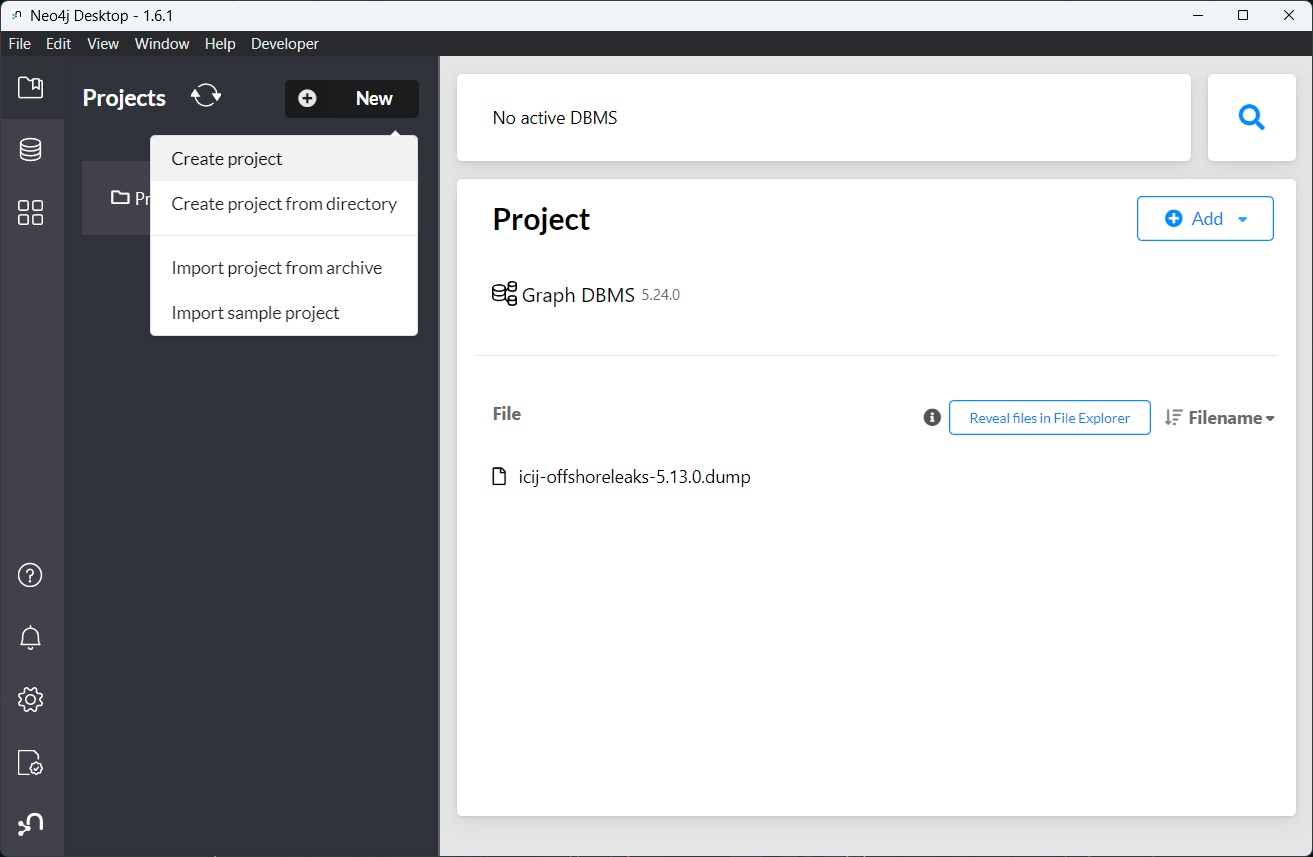
\includegraphics[width=\textwidth]{images/neo4j-setup/1}
        \caption{Creating a project.}
    \end{subfigure}
    \hfill
    \begin{subfigure}[b]{0.49\textwidth}
        \centering
        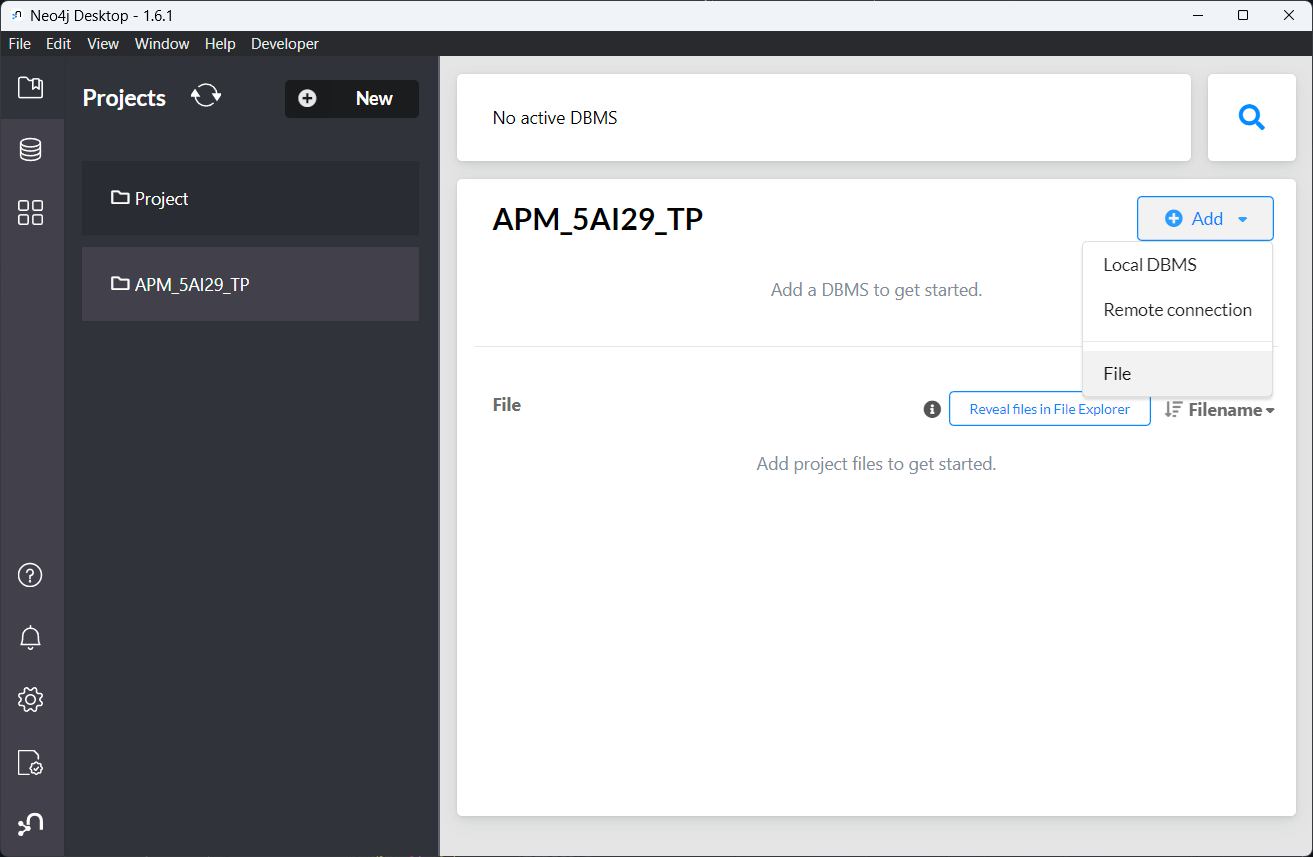
\includegraphics[width=\textwidth]{images/neo4j-setup/2}
        \caption{Adding dump file.}
    \end{subfigure}
    \\
    \begin{subfigure}[b]{0.49\textwidth}
        \centering
        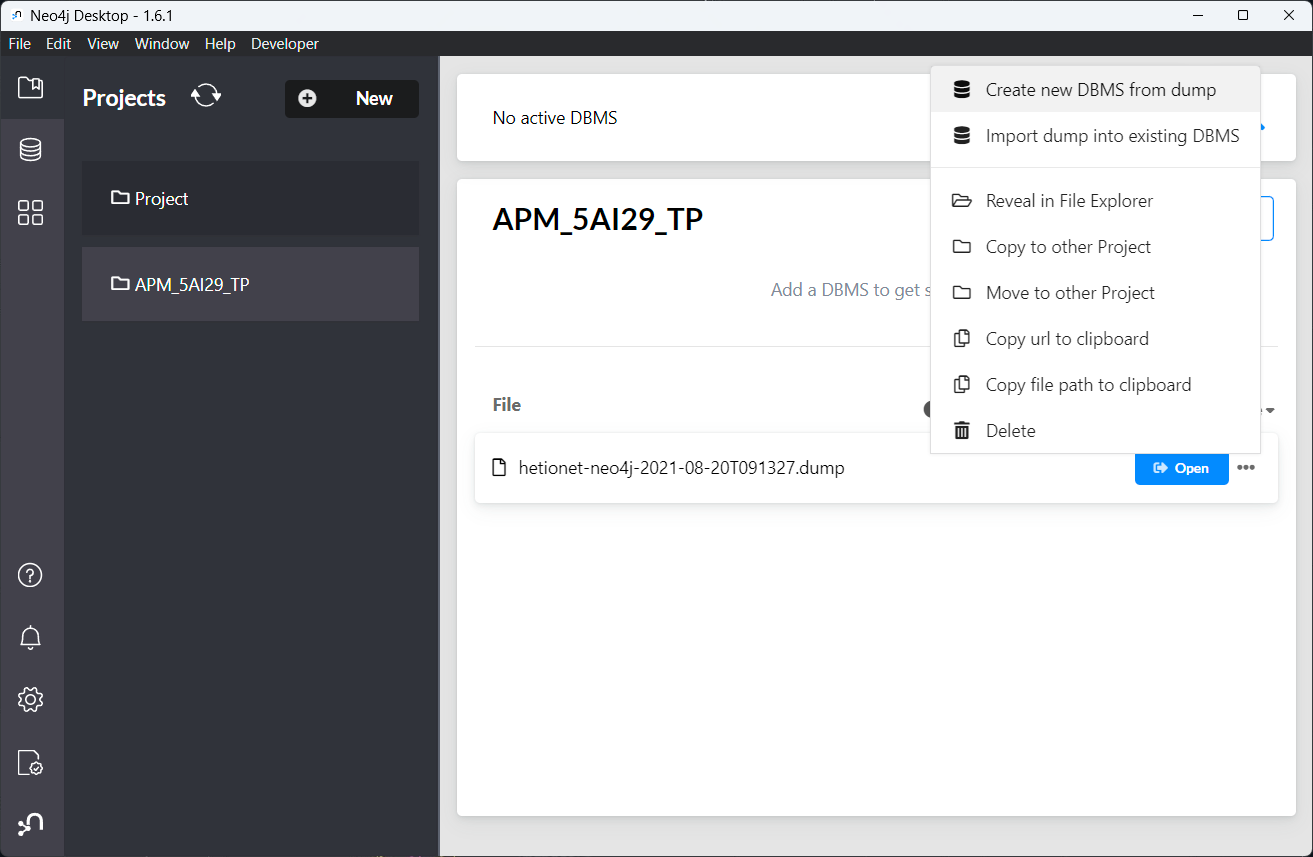
\includegraphics[width=\textwidth]{images/neo4j-setup/3}
        \caption{Importing dump to DBMS.}
    \end{subfigure}
    \hfill
    \begin{subfigure}[b]{0.49\textwidth}
        \centering
        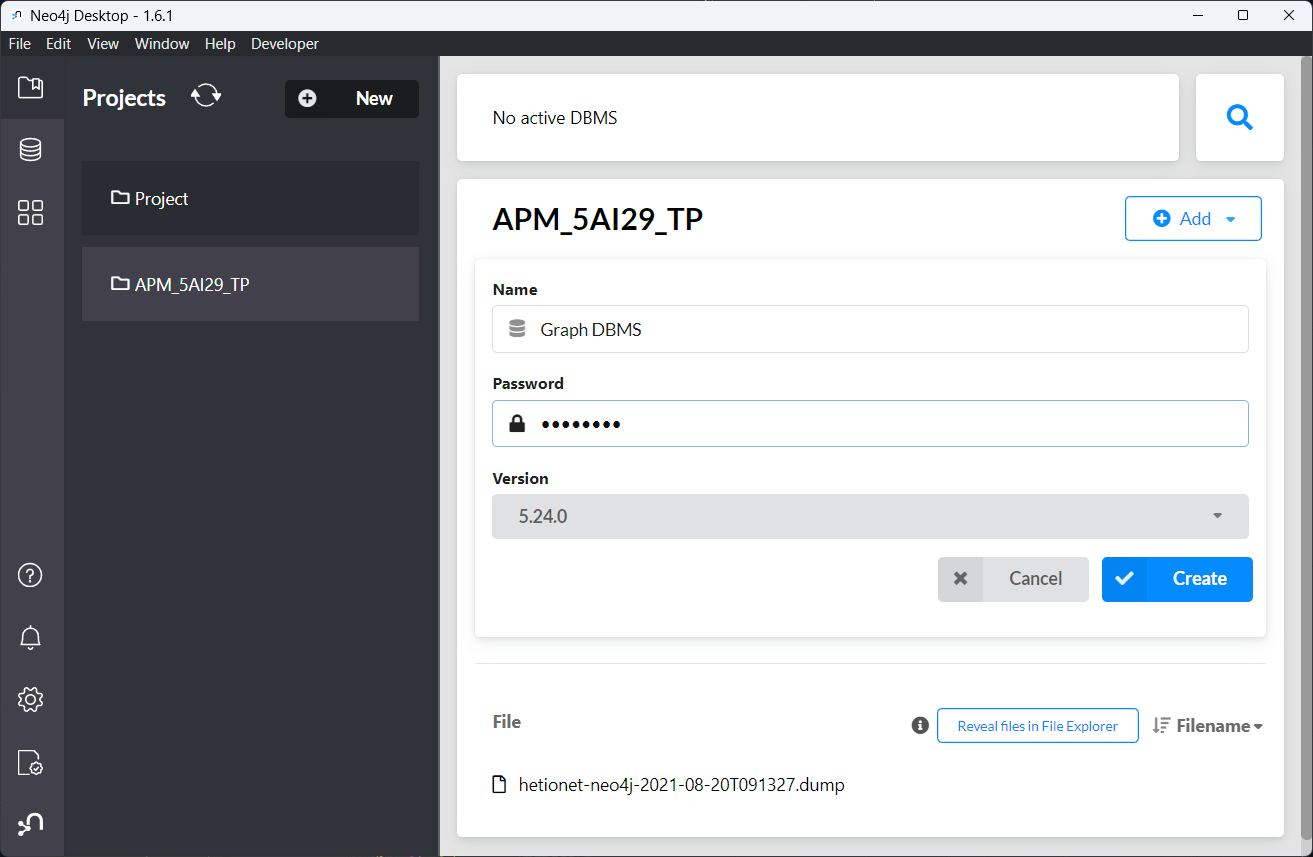
\includegraphics[width=\textwidth]{images/neo4j-setup/4}
        \caption{Configuring DBMS.}
    \end{subfigure}
    \\
    \begin{subfigure}[b]{0.49\textwidth}
        \centering
        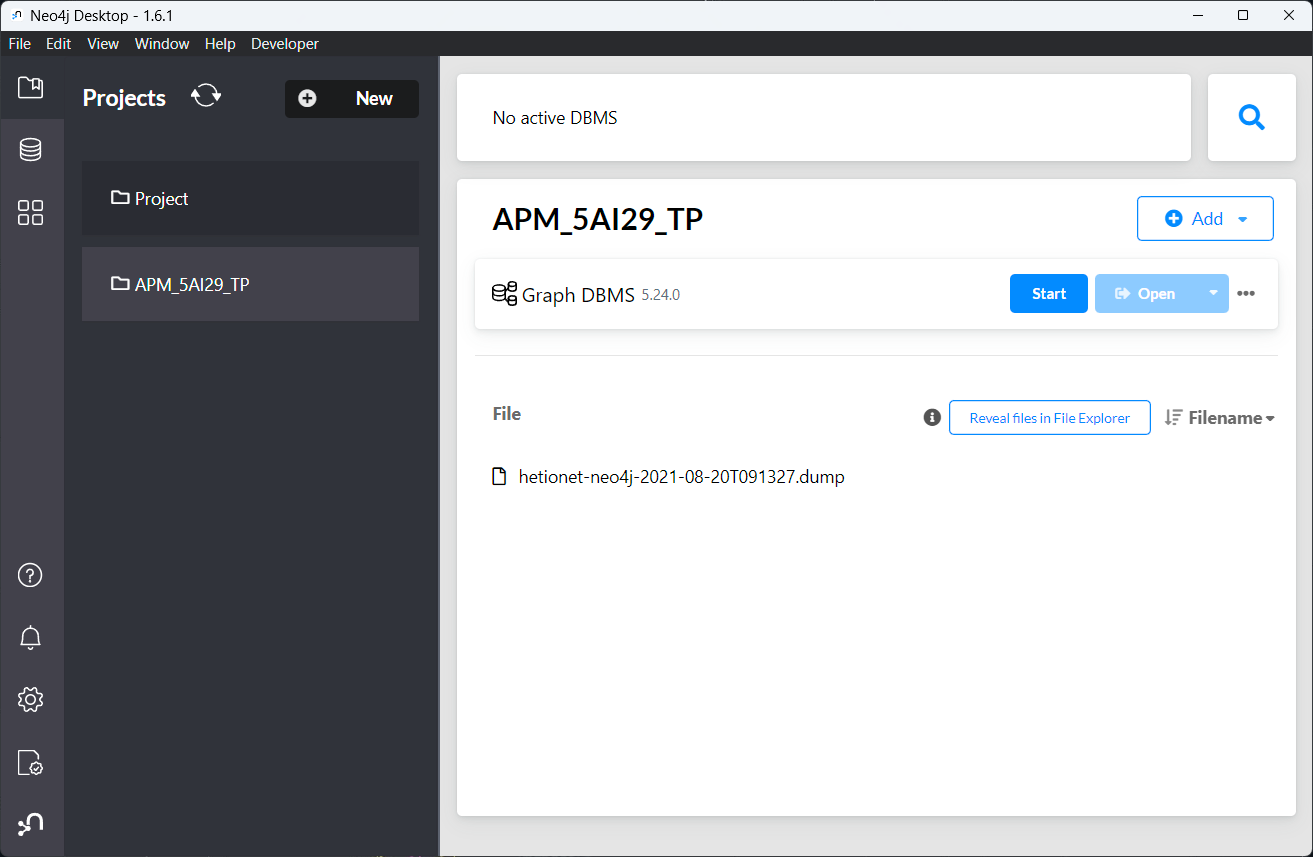
\includegraphics[width=\textwidth]{images/neo4j-setup/5}
        \caption{Starting DBMS.}
    \end{subfigure}
    \hfill
    \begin{subfigure}[b]{0.49\textwidth}
        \centering
        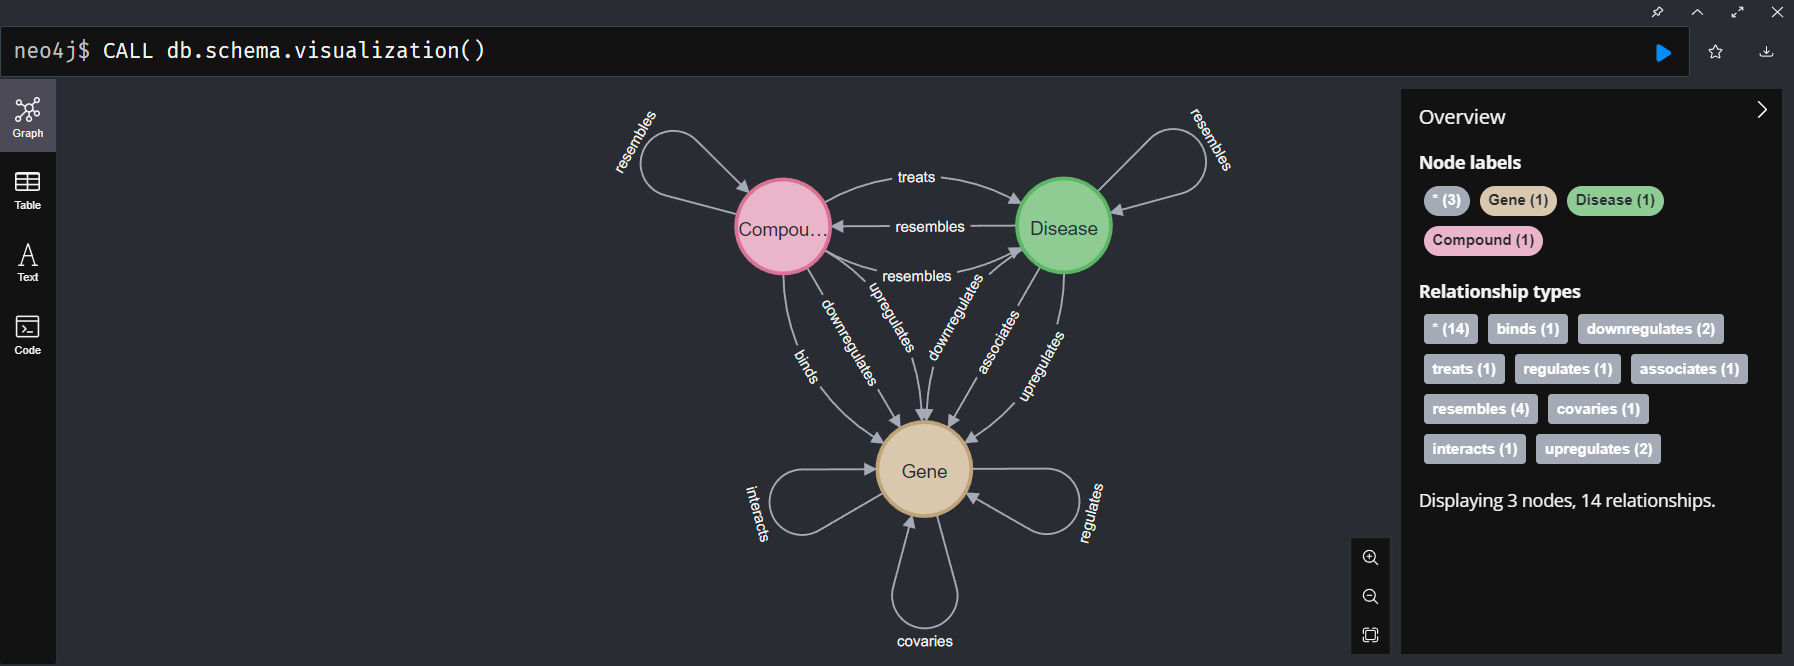
\includegraphics[width=\textwidth]{images/neo4j-setup/7}
        \caption{Visualizing schema.}
    \end{subfigure}

    \caption{Steps for Neo4j Desktop Setup.}
    \label{fig:neo4j-setup}
\end{figure}

Upon successful import, the schema can be visualized using the following Neo4j query: \texttt{CALL db.schema.visualization()}.
The resulting graph, illustrates key entities and relationships that form the basis for multi-class link prediction and knowledge graph completion in subsequent tasks.

\subsection*{Model Evaluation}
\label{model-evaluation}
We evaluated the performance of traditional models and our newly introduced LLM-based approaches for knowledge graph completion.
As a primary baseline, we employed the RotatE model, configured with 128-dimensional embeddings and trained for 100 epochs with early stopping.

For our LLM-based methods, we used the Llama 3.2-3B model, selected for its competitive output quality and relatively low VRAM requirements.
Building upon the RotatE framework, we designed a hybrid architecture that combines 128-dimensional trainable embeddings with 32-dimensional projections of Llama embeddings.
The high-dimensional Llama embeddings (3200 dimensions) are reduced through a trainable linear layer to make them compatible with the RotatE model.

To generate Llama embeddings, we employed two input variants.
The first, referred to as RLM, uses embeddings derived solely from the entity names in the graph.
The second, called RLM-A (RLM Augmented), incorporates Wikidata's retrieval-augmented generation (RAG) technique, providing additional context.
Input labels were tokenized in batches of 32 with a maximum sequence length of 128 tokens.
These tokenized inputs were processed through the Llama model, and embeddings were extracted from the final hidden layer.
Specifically, the hidden state of the first token (analogous to a [CLS] token) was used as a fixed-size vector representation for each label.
These embeddings were stored efficiently on the same device as the model for streamlined processing.

This hybrid approach combines RotatE's ability to learn relational embeddings with Llama's capacity to represent complex label information.
The RLM-A variant further enhances this by incorporating supplementary knowledge from Wikidata entries.


